\newcommand{\adag}[1]{\hat{a}_{#1}^\dagger}
\newcommand{\aop}[1]{\hat{a}_{#1\vphantom{\dagger}}}
\chapter{Theory: Background}
This chapter will cover the elementary concepts required to describe an membrane based optomechanical system in a quantum regime. We will first recall basics on optical field quantization as well describing coherent and squeezed light field, to then turn to the more specific frequency dependent squeezed light field. Secondly, we will cover the mathematical description of a mechanical resonator interacting with a generic coherent optical field, highlighting the differences with the seminal optomechanical system of a mirror on a spring. Finally, we will derive the equations of motions of a membrane based optomechanical system with frequency dependent squeezed optical fields. 
\minitoc
\newpage
\section{Quantum Optics}
\subsection{Quantum Description of Light}

\subsubsection{Quantised Electromagnetic Field}
% \the\textwidth
We consider the quantised electromagnetic field in a volume $V$. The electric field operator can be written as  
\begin{equation}
\hat{\mathbf{E}}(\mathbf{r}, t) 
= i \sum_{\ell} \mathcal{E}_\ell 
\left[ \hat{a}^{\vphantom{\dagger}}_{\ell}\,\mathbf{f}_{\ell}(\mathbf{r})\,e^{-i\omega_{\ell} t} 
- \hat{a}_{\ell}^\dagger\,\mathbf{f}_{\ell}^*(\mathbf{r})\,e^{+i\omega_{\ell} t} \right],
\end{equation}
where   $\mathcal{E}_l = \sqrt{\frac{\hbar \omega_l}{2 \varepsilon_0 V}}$ is the field amplitude per photon in mode $\ell$, $\hbar$ is the reduced Planck constant, $\omega_\ell$ is the angular frequency of mode $\ell$, and $\varepsilon_0$ is the vacuum permittivity. The spatial mode functions $\mathbf{f}_{\ell}(\mathbf{r})$ form an orthonormal basis in $V$ according to  
\begin{equation*}
\int_V d^3r\; \mathbf{f}_{\ell}^*(\mathbf{r}) \cdot \mathbf{f}_{\ell'}(\mathbf{r}) 
= \delta_{\ell \ell'} .
\end{equation*}
The annihilation and creation operators $\hat{a}_{\ell}(t)$ and $\hat{a}_{\ell}(t)^\dagger$ satisfy the canonical commutation relations  
\[
[\hat{a}_{\ell}^{\vphantom{\dagger}}, \hat{a}_{\ell'}^\dagger] = \delta_{\ell \ell'} \,, \quad
[\hat{a}_{\ell}^{\vphantom{\dagger}}, \hat{a}_{\ell'}^{\vphantom{\dagger}} ] = 0, \quad [\hat{a}_{\ell}^\dagger, \hat{a}_{\ell'}^\dagger] = 0  
\]
The explicit time dependence of the operators allows one to describe both slow classical modulations of the field and the intrinsic quantum fluctuations.

\subsubsection{Fock basis}
In this description of the optical field, each mode $\ell$ is modeled as a quantum harmonic oscillator with a discrete set of energy eigenstates known as \textit{Fock states} or number states, denoted $\ket{n_\ell}$. These states form an orthonormal basis and satisfy $\hat{n}_{\ell} \ket{n_\ell} = n_\ell \ket{n_\ell}$, where $\hat{n}_{\ell}$ is the number operator defined by
\[
\hat{n}_{\ell} = \hat{a}_{\ell}^\dagger \hat{a}^{\vphantom{\dagger}}_{\ell}.
\]
The action of the creation and annihilation operators on these states is given by
\[
\hat{a}^{\vphantom{\dagger}}_{\ell} \ket{n_\ell} = \sqrt{n_\ell} \ket{n_\ell - 1}, \quad
\hat{a}_{\ell}^\dagger \ket{n_\ell} = \sqrt{n_\ell + 1} \ket{n_\ell + 1}.
\]
They allow transitions between Fock states by lowering or raising the photon number in mode $\ell$ by one unit. The vacuum state $\ket{0_\ell}$ is annihilated by $\hat{a}^{\vphantom{\dagger}}_{\ell}$, satisfying $\hat{a}^{\vphantom{\dagger}}_{\ell} \ket{0_\ell} = 0$. Thus, the Hamiltonian for the electromagnetic field becomes a sum of harmonic oscillator energies:
\begin{equation}
\hat{H} = \sum_\ell \hbar \omega_{\ell} \, \hat{a}_{\ell}^\dagger \hat{a}^{\vphantom{\dagger}}_{\ell} 
\end{equation}
where we ignore the constant zero-point energy term $\frac{1}{2} \hbar \omega_{\ell}$ for simplicity. \\

In the following parts, we will always focus on a single mode of the electromagnetic field unless stated otherwise (for the mode matching part), which is sufficient to illustrate the concepts of quantum optics and optomechanics. The generalization to multiple modes is straightforward and follows the same principles. The electrif field operator is then written
\begin{equation}
\hat{\mathbf{E}}(\mathbf{r}, t)
= i \mathcal{E}_0
\left[ \hat{a}^{\vphantom{\dagger}}\,\mathbf{f}(\mathbf{r})\,e^{-i\omega_0 t}
- \hat{a}^\dagger\,\mathbf{f}^*(\mathbf{r})\,e^{+i\omega_0 t} \right].
\end{equation}


\subsubsection{Quadrature Operators}
We describe the phase-space properties of a field mode using hermitian quadrature operators. These are linear combinations of the annihilation and creation operators that correspond to measurable observables in the electromagnetic field. The two most common quadratures are defined as follows:
\begin{equation}
\mathbf{\hat{a}}\;\equiv\;
\begin{pmatrix}\hat a_1\\[2pt]\hat a_2\end{pmatrix}
=\mathbf\Gamma \, \mathbf{\hat{u}}, \label{II.2}
\qquad
\mathbf \Gamma \equiv
\begin{pmatrix}
1 & 1 \\
-i & i
\end{pmatrix},
\quad
\mathbf{\hat{u}}\;\equiv\;
\begin{pmatrix}\hat a\\ \hat a^\dagger\end{pmatrix}
\end{equation}
where we defined the field vector $\mathbf{\hat{u}}$ and the transfer matrix $\mathbf \Gamma$, later used to switch from One-Photon to Two-Photon description of optical elements. In components, we then have $\hat a_1=\hat a^\dagger+\hat a$ and $\hat a_2=i(\hat a^\dagger-\hat a)$.
The matrix form commutator reads
\begin{equation}
[\mathbf{\hat{u}}, \mathbf{\hat{u}}^{\dagger}] = \mathbf{\sigma_z}, 
\end{equation}
with $\sigma_z$ the Pauli Z matrix. 
An arbitrary rotated quadrature pair is obtained by
\begin{equation}
\mathbf{\hat{a}_\phi}\;\equiv\;
\begin{pmatrix}\hat a_\phi\\[2pt]\hat a_{\phi+\pi/2}\end{pmatrix}
= \mathbf R(\phi)\,\mathbf{\hat{a}}
= \mathbf R(\phi)\,\mathbf\Gamma \,\mathbf{\hat{u}},
\qquad
 \mathbf R(\phi)\equiv
\begin{pmatrix}
\cos\phi & \sin\phi \\
-\sin\phi & \cos\phi \label{II.4}
\end{pmatrix}.
\end{equation}
We notice than 
\begin{equation}
\mathbf R(\phi)\,\boldsymbol{\Gamma}
=
\begin{pmatrix}
\cos\phi & \sin\phi \\
-\sin\phi & \cos\phi
\end{pmatrix}
\begin{pmatrix}
1 & 1 \\
-i & i
\end{pmatrix}
=
\begin{pmatrix}
e^{-i\phi} & e^{i\phi} \\[4pt]
-\,i\,e^{-i\phi} & \;\;i\,e^{i\phi}
\end{pmatrix}.
\end{equation}
so that in components we have 
\begin{equation}
\begin{alignedat}{3}
\hat a_\phi \;&=\;& \hat a_1 \cos\phi + \hat a_2 \sin\phi \;&= \hat a\,e^{-i\phi} + \hat a^\dagger\,e^{+i\phi}\\
\hat a_{\phi+\pi/2} \;&=\;& -\hat a_1 \sin\phi + \hat a_2 \cos\phi \;&= i\!\left(\hat a^\dagger\,e^{+i\phi} - \hat a\,e^{-i\phi}\right).
\end{alignedat}
\end{equation}
The commutators of the rotated quadrature operators read
\begin{equation}
\begin{aligned}
[\hat{\mathbf{a}}_\phi , \hat{\mathbf{a}}_\phi^{\dagger}]
&= \mathbf R(\phi) \mathbf \Gamma\,[\hat{\mathbf{u}},\hat{\mathbf{u}}^{\dagger}]\, \mathbf \Gamma^{\dagger} \mathbf R^{\dagger}(\phi) \\[4pt]
&= \mathbf R(\phi)\mathbf \Gamma \mathbf \sigma_z \mathbf \Gamma^{\dagger} \mathbf R^{\dagger}(\phi) \\[4pt]
&= 2i\, \mathbf R(\phi) \mathbf J \mathbf R^{\dagger}(\phi) \\[4pt]
&= 2i\,\mathbf J,
\end{aligned}
\end{equation}
where $\mathbf{J}$ is the symplectic form defined as
\begin{equation}
\mathbf{J} \equiv
\begin{pmatrix}
0 & 1 \\
-1 & 0
\end{pmatrix}.
\end{equation}
Note that since $\hat{\mathbf{a}}_\phi$ is hermitian, we have $\hat{\mathbf{a}}_\phi^\dagger = \hat{\mathbf{a}}_\phi^T$, and similarly $\mathbf{R^\dagger(\phi)} = \mathbf{R}^T(\phi)$ since all its entries are real. \\ 
\\
This compact vector form will be used later for the one- and two-photon description of the light field behaviours in optomechanical systems with squeezed light input. \\
\noindent \textbf{Note:} \color{red} notes the fact that these are defined for a specific $\ell$, so at each mode is associated such a quadrature vector. The multimode treatment is used by the multimode quantum optics community, notably to describe mutimode non gaussian states, hidden squeezing (beyond homodyne detection correlations, Patera and co) \color{black}
\subsubsection{Linearization of the optical field}

The annihilation operator can be decomposed as
\begin{equation}
\begin{split}
    \hat{a} & = \langle \hat{a} \rangle + \delta\hat{a}\\
    & = \bar{\alpha} + \delta\hat{a} \\
\end{split}
\label{II.8}
\end{equation}
where \(\langle \hat{a} \rangle = \bar{\alpha} \in \mathbb{C}\) is the mean complex amplitude of the quantum state, and \(\delta\hat{a}\) represents quantum fluctuations with \(\langle \delta\hat{a}\rangle = 0\). Note this decomposition is valid for any quantum state, including coherent and squeezed states. We note $\bar{\alpha}$ to distinguish it from the complex amplitude $\alpha$ of a coherent state introduced below, which is a specific case of this decomposition. The associated matrix form is 
\begin{equation}
\mathbf{\hat{u}} =  \begin{pmatrix} \bar{\alpha}  \\ \bar{\alpha}^*  \end{pmatrix} + \begin{pmatrix} \delta\hat{a} \\ \delta\hat{a}^\dagger \end{pmatrix} =  \mathbf{\bar{u}} + \mathbf{\delta \hat{u}}
\end{equation}
and it then follows that the quadrature operators can also be expressed as
\begin{equation}
  \begin{split}
    \mathbf{\hat{a}_\phi} & = \mathbf{R}(\phi) \, \mathbf\Gamma  \,(\mathbf{\bar{u}} + \mathbf{\delta \hat{u}}) \\
    & = \mathbf{\bar{a}_\phi}  + \mathbf{\delta \hat{a}_\phi} 
  \end{split}
\end{equation}
where the fluctuations retain the canonical commutation relations
\begin{equation}
[\mathbf{\delta \hat{u}}, \mathbf{\delta \hat{u}}^{\dagger}] = \mathbf{\sigma_z} \qquad \Rightarrow \qquad
[\mathbf{\delta \hat{a}_\phi}, \mathbf{\delta \hat{a}_\phi}^{T}] = 2i\,\mathbf{J}.
\label{II.11}
\end{equation}

\noindent \textbf{Note:} \color{red} notes on first and second moments, as well as beyond second moments correlations and their use i.e. when and why is this linearization ok to use etc etc \color{black}

\subsubsection{Heisenberg Uncertainty Relation }
The covariance of Hermitian operators \(\hat{A}\) and \(\hat{B}\) is defined as
\begin{equation}
    \mathrm{Cov}(\hat{A},\hat B) = \tfrac12 \big\langle \{ \delta\hat{A}, \delta\hat{B} \} \big\rangle \\
\end{equation}
such that it reduces to the variance $\delta A^2$ if $\hat{A}=\hat{B}$. Considering the quadrature operators, we define the covariance matrix as
\begin{equation}
\mathbf{V_\phi} \equiv \tfrac12 \big\langle \{  \mathbf{\delta \hat{a}_\phi},  \mathbf{\delta \hat{a}_\phi}^{\,T} \} \big\rangle
= \begin{pmatrix}
\langle \delta \hat{a}_\phi^2 \rangle &
\mathrm{Cov}(\hat{a}_\phi,\hat{a}_{\phi+\pi/2}) \\[4pt]
\mathrm{Cov}(\hat{a}_\phi,\hat{a}_{\phi+\pi/2})  &
\langle \delta \hat{a}_{\phi+\pi/2}^2 \rangle 
\end{pmatrix}
\end{equation}
and the Heisenberg uncertainty relation reads as
\begin{equation}
  \det \mathbf{V_\phi} \geq 1 \qquad \Rightarrow \qquad \langle  \delta \hat{a}^2_\phi \rangle \langle  \delta \hat{a}^2_{\phi+\pi/2} \rangle  - \mathrm{Cov}^2(\hat{a}_\phi,\hat{a}_{\phi+\pi/2})\geq 1
\end{equation}


\subsubsection{Graphical Representation of Gaussian States}
For Gaussian states, we can actually picture them in a 2D space, where ... 

\subsection{Coherent and Squeezed States}
We now turn to standard optical quantum states, in particular gaussian states i.e.\ full positive in Wigner function representations such as coherent and squeezed states, that we will denote in braket notation as $|\alpha\rangle$ and $|\alpha,r, \theta\rangle $.
\subsection*{Coherent States:}
The coherent state $\ket{\alpha}$ is an eigenstate of the annihilation operator:
\begin{equation}
\hat{a}\ket{\alpha} = \alpha \ket{\alpha}
\label{II.14}
\end{equation}
where $\alpha = |\alpha| e^{i\bar{\varphi}}$ is a complex number representing the mean coherent amplitude. In this notation, the angle $\bar{\varphi}$ is the mean angle of the distribution, used to describe the relative phase to a reference (e.g. a local oscillator), as in Fig ??. The $\hat{a}$ linear decomposition above (Eq~\eqref{II.8}) then yields $\alpha = \bar{\alpha}$ for a coherent state. It can be expressed in the Fock basis as
\begin{equation}
\ket{\alpha} = e^{-|\alpha|^2/2} \sum_{n=0}^\infty \frac{\alpha^n}{\sqrt{n!}}\,\ket{n}
\label{II.15}
\end{equation}
and are generated by the action of the displacement operator $\hat{D}(\alpha)$ on the vacuum state $\ket{0}$:
\begin{equation}
\ket{\alpha} = \hat{D}(\alpha)\ket{0},\qquad \hat{D}(\alpha) = \exp\!\left(\alpha \hat{a}^\dagger - \alpha^* \hat{a}\right)
\label{II.16}
\end{equation}
\noindent \textbf{Note:} \color{red} note on the convention used i.e. $\alpha \neq \bar{\alpha}$, $\alpha_0 \neq \bar{\alpha}_0$ \color{black}
\subsubsection*{Expectation values of quadrature operators}

Using the quadrature vector $\hat{\mathbf{a}}_\phi$ (Eq~\ref{II.4}), the expectation values in a coherent state are
\begin{equation}
\langle \hat{\mathbf a}_\phi\rangle
= \mathbf R(\phi)\,\langle \hat{\mathbf a}\rangle
=
2\begin{pmatrix}
\mathrm{Re}\big(\alpha e^{-i\phi}\big) \\[2pt]
\mathrm{Im}\big(\alpha e^{-i\phi}\big)
\end{pmatrix}
\end{equation}
such that the components reduce to $2\mathrm{Re} (\alpha)$ and  $2\mathrm{Im} (\alpha)$ if $\phi=0$. 

\subsubsection*{Amplitude and phase quadratures}

It is convenient to introduce the amplitude-phase quadrature vector at $\phi = \bar{\varphi}$
\begin{equation}
\hat{\mathbf a}_{\bar{\varphi}} =
\begin{pmatrix}
\hat{p} \\[2pt]
\hat{q}
\end{pmatrix}
=
\begin{pmatrix}
\hat{a}_{\bar{\varphi}} \\[2pt]
\hat{a}_{\bar{\varphi}+\pi/2}
\end{pmatrix}.
\end{equation}
with expectation values
\begin{equation}
\langle \hat{\mathbf a}_{\bar{\varphi}} \rangle
=
2\begin{pmatrix}
|\alpha| \\[2pt]
0
\end{pmatrix},
\end{equation}



\subsubsection*{Covariance matrix}
For a coherent state, fluctuations are vacuum-like:
\begin{equation}
\delta \hat{a}_\phi^2 = \delta \hat{a}_{\phi+\pi/2}^2 = 1,
\qquad
\mathrm{Cov}(\hat{a}_\phi,\hat{a}_{\phi+\pi/2}) = 0,
\end{equation}
so that
\begin{equation}
\mathbf V_\phi =
\begin{pmatrix}
1 & 0\\
0 & 1
\end{pmatrix}
= \mathbb{I}_2,
\quad \forall \phi .
\label{II.CS.3}
\end{equation}
This saturates the Heisenberg uncertainty relation $\det \mathbf V_\phi = 1$ in the units defined here i.e. it is a minimum uncertainty state. 

\subsubsection*{Photon number statistics}

The mean and variance of the photon number operator $\hat{N}=\hat{a}^\dagger\hat{a}$ are
\begin{equation}
\langle \hat{N} \rangle = |\alpha|^2,
\qquad
\Delta N^2 = |\alpha|^2.
\label{II.19}
\end{equation}
That is, coherent states display Poissonian photon statistics.


\begin{figure}
\centering
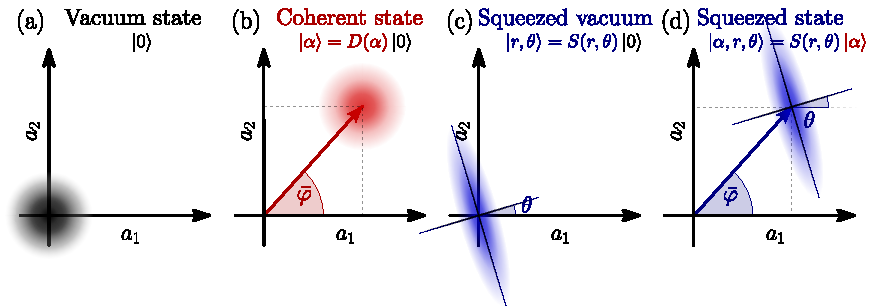
\includegraphics[width=\textwidth]{./chap2/fig/quantum_states.pdf}
\caption{Phase-space representations of quantum states and transformations.
(a) Wigner function of the vacuum state: a circular Gaussian centered at the origin, representing equal quantum fluctuations in both quadratures $a_1$ and $a_2$.
(b) Wigner function of a coherent state: a displaced circular Gaussian, showing a shift in phase space along an angle $\varphi$ with unchanged, isotropic noise.
(c) Wigner function of a squeezed vacuum state: an elliptical Gaussian centered at the origin, with reduced noise along a rotated quadrature $X_\theta$ and increased noise in the orthogonal direction.
(d) Wigner function of a displaced squeezed state: an ellipse shifted away from the origin, combining anisotropic fluctuations and a nonzero mean amplitude. The displacement angle $\varphi$ and squeezing angle $\theta$ are independent.} 
\end{figure}


\subsection*{Squeezed States:}

Squeezed states $|\alpha, r, \theta\rangle $ are quantum gaussian states of light in which the noise (variance) of one quadrature is reduced below the vacuum level, at the expense of increased noise in the conjugate quadrature. The single-mode squeezed vacuum state is defined as
\begin{align}
|0, r, \theta \rangle = \hat{S}(r, \theta) |0\rangle , \quad \hat{S}(\theta) = \exp\left[\frac{r}{2}(e^{-2 i\theta} \hat{a}^2 - e^{-2 i\theta} \hat{a}^{\dagger 2})\right]
\end{align}
where $r$ is the squeezing parameter (strength) and $\theta$ is the squeezing angle i.e. the angle along which one quadrature is reduced below vacuum level. The most general Gaussian state is the displaced squeezed state, obtained by applying both the squeezing operator $\hat{S}(r, \theta)$ and the displacement operator $\hat{D}(\alpha)$ to the vacuum:
\begin{equation}
|\alpha, r, \theta\rangle = \hat{S}(r, \theta)\hat{D}(\alpha)|0\rangle
\end{equation}
where $\hat{D}(\alpha)$ displaces the state in phase space by the complex amplitude $\alpha$, defined similarly to the coherent state. \\

\noindent \textbf{Note:}  The displacement and squeezing operators do not commute, i.e. $\hat{D}(\alpha)\hat{S}(r, \theta) \neq \hat{S}(r, \theta)\hat{D}(\alpha)$. However, both orderings correspond to experimentally valid procedures: one can either squeeze the vacuum and then displace (e.g. by mixing with a coherent state ona beamsplitter), or squeeze a coherent state straight away (e.g. by seeding an optical parametric amplifier). The resulting state is always a displaced squeezed state, but the relative phase between displacement and squeezing may differ.
% -------------------------------------------------
\subsubsection*{Expectation values of quadrature operators}

Using the usual quadratures defined in Eq~\eqref{II.2} and \eqref{II.4}, the expectation values in a displaced squeezed state are
\begin{equation}
\langle \mathbf{\hat{a}} \rangle
= 2
\begin{pmatrix}
\mathrm{Re}\,\alpha \\[2pt]
\mathrm{Im}\,\alpha
\end{pmatrix}, 
\qquad
\langle \mathbf{\hat{a}_\phi} \rangle
= 2
\begin{pmatrix}
\mathrm{Re}\!\left(\alpha e^{-i\phi}\right) \\[2pt]
\mathrm{Im}\!\left(\alpha e^{-i\phi}\right)
\end{pmatrix}.
\label{II.xx3}
\end{equation}
For a squeezed vacuum ($\alpha=0$) all quadrature means vanish.

\subsubsection*{Quadrature aligned with the squeezing axis \color{red} to rewrite \color{black}}

Choosing $\phi = \theta$ yields
\begin{equation}
\langle \delta \hat a_\theta^2  \rangle = e^{-2r}, \qquad
\langle \delta \hat a_{\theta+\pi/2}^2 \rangle = e^{2r}, \qquad
\mathrm{Cov}(\hat a_\theta, \hat a_{\theta+\pi/2}) = 0,
\end{equation}
with uncertainty product $\Delta \hat a_\theta\, \Delta \hat a_{\theta+\pi/2} = 1$ saturating the Heisenberg bound.
The corresponding mean vector is
\begin{equation}
\langle \mathbf{\hat{a}_\theta} \rangle
= 2
\begin{pmatrix}
\mathrm{Re}(\alpha e^{-i\theta}) \\[2pt]
\mathrm{Im}(\alpha e^{-i\theta})
\end{pmatrix}.
\label{II.xx7}
\end{equation}

\begin{figure}
\centering
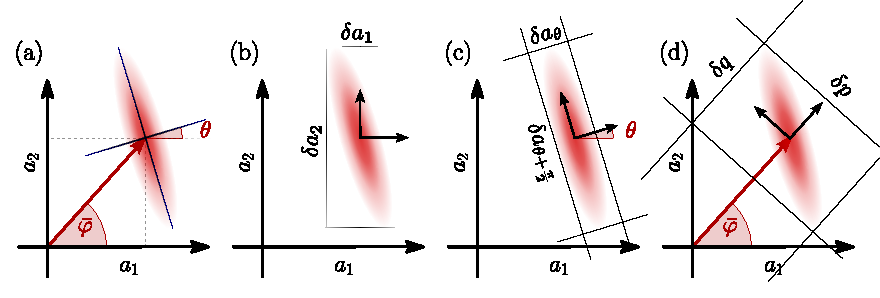
\includegraphics[width=\textwidth]{./chap2/fig/quantum_quadraturesBis.pdf}
\caption{Phase-space representations of quantum states and transformations.
(a) Wigner function of the vacuum state: a circular Gaussian centered at the origin, representing equal quantum fluctuations in both quadratures $X_1$ and $X_2$.
(b) Wigner function of a coherent state: a displaced circular Gaussian, showing a shift in phase space along an angle $\varphi$ with unchanged, isotropic noise.
(c) Wigner function of a squeezed vacuum state: an elliptical Gaussian centered at the origin, with reduced noise along a rotated quadrature $X_\theta$ and increased noise in the orthogonal direction.
(d) Wigner function of a displaced squeezed state: an ellipse shifted away from the origin, combining anisotropic fluctuations and a nonzero mean amplitude. The displacement angle $\varphi$ and squeezing angle $\theta$ are independent.} 
\end{figure}
% -------------------------------------------------
\subsubsection*{Covariance matrix}

Let $\psi \equiv \phi - \theta$ be the measurement angle $\phi$ relative to the squeezing axis $\theta$.  
For a displaced squeezed state, the covariance matrix is
\begin{equation}
\mathbf{V}_\phi = \mathbf R(\psi)
\begin{pmatrix}
e^{-2r} & 0 \\[2pt]
0 & e^{2r}
\end{pmatrix}
\mathbf R(\psi)^{T}.
\label{II.xx4}
\end{equation}
Expanding this explicitly gives
\begin{equation}
\mathbf{V}_\phi =
\begin{pmatrix}
e^{-2r} \cos^2\!\psi + e^{2r} \sin^2\!\psi 
& \frac{1}{2} \sin 2\psi \,\left(e^{2r} - e^{-2r}\right) \\[6pt]
\frac{1}{2} \sin 2\psi \,\left(e^{2r} - e^{-2r}\right) 
& e^{-2r} \sin^2\!\psi + e^{2r} \cos^2\!\psi
\end{pmatrix}.
\label{II.xx5}
\end{equation}
The covariance term is therefore
\begin{equation}
\mathrm{Cov}(\hat a_\phi, \hat a_{\phi+\pi/2})
= \frac{1}{2} \sin 2(\phi-\theta)\, \left(e^{2r} - e^{-2r}\right),
\label{II.xx6}
\end{equation}
which vanishes when $\sin 2(\phi-\theta) = 0$, i.e.
\begin{equation*}
\phi - \theta \in \left\{ 0, \frac{\pi}{2}, \pi, \ldots \right\}.
\end{equation*}
Along these principal axes of squeezing, $\mathbf{V}_\phi$ is diagonal. 

\subsubsection{Amplitude and Phase squeezed states}
Considering a displaced squeezed state, two special cases are of interest: the amplitude squeezed state where $\theta=\bar{\varphi}$ and the phase squeezed state where $\theta = \bar{\varphi}+\pi/2$. In the first case, the amplitude quadrature $\hat{p}$ is squeezed, while the phase quadrature $\hat{q}$ is anti-squeezed. In the second case, the phase quadrature is squeezed, while the amplitude quadrature is anti-squeezed. The covariance matrices for these states can be derived from Eq.~\eqref{II.xx4} by setting $\psi = 0$ or $\psi = \pi/2$, respectively.
\subsubsection*{Photon number statistics}

The mean and variance of the photon number operator $\hat N = \hat a^\dagger \hat a$ in a displaced squeezed state are
\begin{equation}
\langle \hat N \rangle = |\alpha|^2 + \sinh^2 r,
\qquad
\Delta N^2 = |\alpha|^2 \cosh 2r + \frac{1}{2} \sinh^2 2r.
\label{II.xx8}
\end{equation}
\color{red}
to rewrite
\color{black}
This shows that the squeezing operation increases the mean photon number of the coherent state by adding photons. Physically, this reflects the fact that generating squeezed light requires injecting energy into the system, so the squeezed vacuum contains correlated field excitations (photons) in even numbers. This is further seen by examining the photon-number distribution $P_n$: for a squeezed vacuum only even $n$ occur, while displacement progressively repopulates the odd $n$ and shifts weight to higher $n$, in agreement with the increase of $\langle \hat{N} \rangle$ and $\Delta N^2$ above.



\color{black}

\subsection{Sidebands and Quantum Noises}

\subsubsection{Modulation picture}
In realistic optical systems, the electromagnetic field is never perfectly monochromatic, nor isolated from its environment, nor static through time. Instead, it exhibits a finite spectral linewidth (stimulated emission, phase noise etc...), as well as non intentional/intentional modulations, all imprinted onto the carrier field. These effects cause the field amplitude and phase to evolve slowly compared to the optical frequency $\omega_0$. \\

As a result, the complex amplitude associated with each mode and described by the Schrodinger-picture annihilation operator $\hat{a}$, acquires an explicit time dependence beyond the standard fast-oscillating term $e^{-i\omega_0 t}$. It is often quoted as \textit{modulation} picture in the litterature. We then promote the field vector to 
\begin{equation}
\mathbf{\hat{u}}= \mathbf{\bar{u}} + \mathbf{\delta \hat{u}} \quad \rightarrow \quad
  \mathbf{\hat{u}}(t)=
 \mathbf{\bar{u}}(t) + \mathbf{\delta \hat{u}(t)}
\end{equation}
where the canonical commutation relations given in equation~\eqref{II.11} becomes:
\begin{equation}
  [\delta\mathbf{\hat{u}}(t), \delta \mathbf{\hat{u}}(t')^{\dagger}] = \mathbf{\sigma_z} \, \delta (t-t').
\end{equation}
and the covariance matrix of the ammplitude-phase quadratures turns to
\begin{equation}
\mathbf{V}(t, t') = \begin{pmatrix}
\langle \delta \hat{p}(t) \delta \hat{p}(t') \rangle &
\mathrm{Cov}(\hat{p}(t),\hat{q}(t')) \\[4pt]
\mathrm{Cov}(\hat{q}(t),\hat{p}(t'))  &
\langle \delta \hat{q}(t) \delta \hat{q}(t') \rangle 
\end{pmatrix} \delta(t-t')
\end{equation}
This time dependence allows us to track both slow classical modulations of the field $\mathbf{\bar{u}}(t)$ and the intrinsic quantum fluctuations $\mathbf{\delta \hat{u}(t)}$. Note this is equivalent to the interaction picture where the reference angular frequency would be $\omega_0$, but where we also consider dynamical processes way slower than this frequency. Additionally, we will always consider the limit of weak fluctuations, where the quantum noise can be treated perturbatively around the classical field i.e. 
\[
|\bar{\alpha}(t)| \gg \Delta \hat a_\theta(t)
\]
The resulting field operator can then be expressed as a 
\begin{equation}
\begin{aligned}
\hat{\mathbf{E}}(\mathbf{r}, t) 
=i  \mathcal{E}_0 \bigg[ & \left[ \alpha(t)\, \mathbf{f}(\mathbf{r})\, e^{-i \omega_0 t} 
- \alpha^*(t)\, \mathbf{f}^*(\mathbf{r})\, e^{i \omega_0 t} \right] \\
\quad +  &\left[ \delta \hat{a}(t)\, \mathbf{f}(\mathbf{r})\, e^{-i \omega_0 t}
- \delta \hat{a}^\dagger(t)\, \mathbf{f}^*(\mathbf{r})\, e^{i \omega_0 t} \right] \bigg]
\end{aligned}
\end{equation} 

\subsubsection{Fourier Domain \& Sidebands}
To deal with noise spectra, we need to rewrite the various quadratures defined in the previous sections in the Fourier domain, where each frequency component is called a \textit{sideband}.


The Fourier transform of the field vector is defined as
\begin{equation}
  \begin{split}
    \mathbf{\hat{u}}[\Omega] &=\int_{\infty}^{-\infty}  dt \, e^{i\Omega t} \, \mathbf{\hat{u}}(t)\\
\mathbf{\hat{u}}(t) &= \frac{1}{2\pi}\int_{\infty}^{-\infty}  d\Omega \, e^{-i\Omega t} \, \mathbf{\hat{u}}[\Omega]
  \end{split}
\end{equation}
where $\Omega \ll \omega_0$ is the sideband frequency relative to the so called \textit{carrier} frequency $\omega_0$. \color{red}  Add somthing on the true integral bound i.e. bandwidth B  \color{black}In this definition, a notable property is that the hermitian conjugate in the time domain translates to a frequency inversion in the Fourier domain:
\begin{equation}
   \Big[\hat{a}(t)\Big]^{\dagger} = \hat{a}^\dagger(t),  \quad
   \Big[\hat{a}[\Omega]\Big]^{\dagger}  = \hat{a}^\dagger[-\Omega].
\end{equation}
To lighten the notation we will use $\hat{a}^\dagger[\pm\Omega]=\hat{a}_\pm$. Carrying out the linearization in the Fourier domain, we have
\begin{equation}
  \begin{split}
      \mathbf{\hat{u}}[\Omega] &=\begin{pmatrix} \bar{\alpha}_+ \\ \bar{\alpha}^*_- \end{pmatrix} + \begin{pmatrix} \delta\hat{a}_+ \\ \delta\hat{a}^\dagger_- \end{pmatrix} \\
      & = \mathbf{\bar{u}}[\Omega]+ \mathbf{\delta \hat{u}}[\Omega]\\
  \end{split}
\end{equation}
with the fluctuations commutator reading
\begin{equation}
  [\delta \mathbf{\hat{u}}[\Omega], \delta \mathbf{\hat{u}}[\Omega']^{\dagger}] = \mathbf{\sigma_z} \, \delta(\Omega + \Omega').
\end{equation}
The quadrature operators in the Fourier domain are then written as 
\begin{equation}
  \begin{split}
      \mathbf{\hat{a}_\phi}[\Omega] & = \mathbf{R}(\phi) \, \mathbf{\Gamma} \,\mathbf{\bar{u}}[\Omega] + \mathbf{R}(\phi) \, \mathbf{\Gamma} \, \mathbf{\delta \hat{u}}[\Omega] \\
      & = \underbrace{2|\bar{\alpha}| \begin{pmatrix}
  \cos(\bar{\varphi}-\phi) \\[2pt]
  \sin(\bar{\varphi}-\phi)
\end{pmatrix} \delta(\Omega)}_{\text{classical part}} +
\underbrace{\begin{pmatrix}
  \delta \hat{a}_\phi[\Omega] \\[2pt]
\delta \hat{a}_{\phi+\pi/2}[\Omega] \end{pmatrix}}_{\text{quantum fluctuations}}
  \end{split}
\end{equation}
such that the amplitude-phase quadrature vector reads
\begin{equation}
      \mathbf{\hat{a}_{\bar{\varphi}}}[\Omega]  = 2|\bar{\alpha}| \begin{pmatrix}
  1 \\[2pt]
  0
\end{pmatrix} \delta(\Omega) +
\begin{pmatrix}
  \delta \hat{p}[\Omega] \\[2pt]
\delta \hat{q}[\Omega]
\end{pmatrix}
\end{equation}
where we have 
\begin{equation}
  \begin{pmatrix}
  \delta \hat{p}[\Omega] \\[2pt]
\delta \hat{q}[\Omega]
\end{pmatrix} = \begin{pmatrix}
  \delta \hat{a}_+ + \delta \hat{a}^\dagger_-\\[2pt]
i\big(\delta \hat{a}^\dagger_- - \delta \hat{a}_+\big)  
\end{pmatrix}
\label{eq:2photons}
\end{equation}

This very way of writing the field quadratures is known as the \textit{two-photon} formalism, introduced by Caves and Schumaker~\cite{Caves1985,Caves1985a}. Here, we wrote down a vector, linearized form, useful to compute spectra numerically (see section ??). Throughout the litterature, the amplitude-phase two-photon quadratures are called differently, namely $(a_I, a_Q)$ (Caves and Schumaker), $(X_1, X_2)$ (Gerry and Knight), $(X, Y)$ (Bachor and Ralph) or $(x, p)$ (Weedbrook et al.). We chose the $p, q$ convention to perpetuate the convention used at LKB. \\

\noindent\textbf{Note: }
In the modulation picture, fluctuations in the time domain appear as symmetric sidebands at \(+\Omega\) and \(-\Omega\).
Any experimentally accessible, real signal arises from the interference of these two sidebands (quadratures in homodyne detection, intensity fluctuations, photocurrent spectra); equivalently, Hermiticity in time forces Fourier components to couple \(+\Omega\) with \(-\Omega\).
Packaging the field as the two-photon vector \(\big(\hat a[\Omega],\,\hat a^\dagger[-\Omega]\big)^{T}\) therefore groups exactly the two degrees of freedom that generate a single measurable fluctuation at frequency \(\Omega\). This makes correlations between the sidebands (which are the essence of frequency-dependent squeezing) explicit and ensures that quadrature spectra remain manifestly real. By contrast, the vector \(\big(\hat a[\Omega],\,\hat a^\dagger[\Omega]\big)^{T}\) is convenient for per-frequency photon-number or passive-scattering calculations, but it obscures the intrinsic pairing required to form real observables, forcing one to carry \(-\Omega\) separately.
For the noise-spectral analysis pursued here, the sideband-pair representation is thus the phenomenologically natural and algebraically minimal choice.


\subsubsection*{Amplitude Modulation (AM)}

Let the classical amplitude be modulated at $\Omega_{\text{mod}}$ in amplitude:
\begin{equation}
  \alpha(t) = \bar{\alpha} \left(1 + \epsilon_a \cos(\Omega_{\text{mod}} t)\right)
\end{equation}
with $\epsilon_a \ll 1$, the field amplitude modulation depth. While the DC term lives at frequency $\omega_0$, the modulation introduces sidebands at frequencies $\omega_0 \pm \Omega_{\text{mod}}$, seen by expanding the cosine:
\begin{equation}
  \alpha(t) = \bar{\alpha} \Big( 1 + \frac{\epsilon_a }{2}\, e^{i\Omega_{\text{mod}} t} + \frac{\epsilon_a }{2} \,  e^{-i\Omega_{\text{mod}} t} \Big)
\end{equation}


\subsubsection*{Phase Modulation (PM)}
Let the classical amplitude be modulated in phase at frequency $\Omega_{\mathrm{mod}}$:
\begin{equation}
\alpha(t) = \bar{\alpha} \, e^{i \epsilon_{\phi} \cos(\Omega_{\mathrm{mod}} t)}
\label{eq:PM_def}
\end{equation}
with $\epsilon_{\phi} \ll 1$ the field phase modulation depth. Expanding to first order in $\epsilon_{\phi}$ gives:
\begin{equation}
\alpha(t) \approx \bar{\alpha} \Big( 1 + \frac{i \epsilon_{\phi} }{2} \, e^{i\Omega_{\mathrm{mod}} t} + \frac{i \epsilon_{\phi} }{2} \, e^{-i\Omega_{\mathrm{mod}} t} \Big)
\label{eq:PM_expand}
\end{equation}
While the carrier term lives at frequency $\omega_0$, the modulation introduces sidebands at $\omega_0 \pm \Omega_{\mathrm{mod}}$, both shifted in phase by $\pi/2$ relative to the carrier.

\subsubsection{Linearized Hermitian Operators}
In both cases, the field contains a carrier at frequency $\omega$ and two sidebands at $\omega \pm \Omega$. Amplitude modulation results in sidebands that are in phase with the carrier, while phase modulation produces sidebands with a $\pm \pi/2$ phase shift relative to the carrier. We also note a general modulation process as :
\begin{equation}
\alpha(t) = \bar{\alpha} \left(1 + \varepsilon(t) \right)
\end{equation}
where $\varepsilon(t) \in \mathbb{C}$ is a modulation function that weakly modulates the complex amplitude in time, and that features information about the modulation frequency and depth. It then follows that the linearized amplitude-phase operators can be expressed as
\begin{equation}
\hat{\mathbf a}_{\bar{\varphi}} (t) = 2|\bar{\alpha}| \begin{pmatrix}
  1 \\ 0 
\end{pmatrix} + 2|\bar{\alpha}|\begin{pmatrix}
  \mathrm{Re}\big(\varepsilon(t) \big) \\
  \mathrm{Im}\big(\varepsilon(t) \big)
\end{pmatrix}
+ \begin{pmatrix}
  \delta \hat{p}(t) \\
  \delta \hat{q}(t)
\end{pmatrix}
\end{equation}

And the quadrature operators can be expressed as
\begin{equation}
\hat{\mathbf a}_{\bar{\varphi}} [\Omega] =2|\bar{\alpha}| \begin{pmatrix}
  1 \\ 0 
\end{pmatrix}\delta(\Omega) + 2|\bar{\alpha}|\begin{pmatrix}
  \mathrm{Re}\big(\varepsilon[\Omega] \big) \\
  \mathrm{Im}\big(\varepsilon[\Omega] \big)
\end{pmatrix}
+ \begin{pmatrix}
  \delta \hat{p}[\Omega] \\
  \delta \hat{q}[\Omega]
\end{pmatrix}
\end{equation}
Computing the Fourier transform for amplitude and phase modulations yields
\begin{equation}
  \begin{split}
    \varepsilon^{AM}(\Omega) & = \frac{\epsilon_a}{2} \Big(\delta(\Omega - \Omega_{\text{mod}}) +\delta(\Omega + \Omega_{\text{mod}}) \Big)\\
    \varepsilon^{PM}(\Omega) & = \frac{i\epsilon_\phi}{2} \Big(\delta(\Omega - \Omega_{\text{mod}}) + \delta(\Omega + \Omega_{\text{mod}})\Big)
  \end{split}
\end{equation}

\subsubsection{Noise Spectra}
We now introduce the cross spectra matrix for two arbitrary linearized hermitian operators $\hat{A}=\bar{A}+\delta \hat{A}$ and $\hat{B}=\bar{B}+\delta \hat{B}$, which describes their correlations at different frequencies. It is defined as 
\begin{equation}
  \mathbf{S}_{AB}(\Omega) = \begin{pmatrix}
  S_{AA}(\Omega) & S_{AB}(\Omega) \\
  S_{BA}(\Omega) & S_{BB}(\Omega) 
  \end{pmatrix}
\end{equation}
where 
\begin{equation}
   S_{AB}(\Omega) = \frac{1}{2\pi} \int \delta \Omega^{'} \langle \delta \hat{A}(\Omega),\,\delta \hat{B}(\Omega')  \rangle
\label{eq:SAB}
\end{equation}
is the two-sided cross spectrum between $\hat{A}$ and $\hat{B}$. In our way of writing it, we include all time dependent processes inside de fluctuation operators i.e. $\varepsilon(t)$ and $\delta \hat{p}(t)$, $\delta \hat{q}(t)$ in the case of quadrature operators, as all terms in $\delta (\Omega)$ contribute to the DC part of the spectrum. We illustrate this by computing the diagonal elements of the amplitude-phase quadrature of a coherent field modulated in amplitude. The amplitude-phase quadrature fluctuation part reads
\begin{equation}
  \delta \hat{\mathbf a}_{\bar{\varphi}}[\Omega] = |\bar{\alpha}|\epsilon_a \begin{pmatrix}
  \delta(\Omega - \Omega_{\text{mod}}) +\delta(\Omega + \Omega_{\text{mod}}) \\
  0 
\end{pmatrix}
+ \begin{pmatrix}
  \delta \hat{p}[\Omega] \\
  \delta \hat{q}[\Omega]
\end{pmatrix}
\end{equation}
and its amplitude and phase noise spectra are
\begin{equation}
  \begin{split}
    S_{pp}(\Omega) & = 2|\bar{\alpha}|^2 \epsilon_a^2 \Big(\delta(\Omega - \Omega_{\text{mod}}) +\delta(\Omega + \Omega_{\text{mod}}) \Big) + 1\\
    S_{qq}(\Omega) & = 1
  \end{split}
\end{equation}





\subsection{Quantum Sideband Diagram }
As seen in the above expression for the amplitude and phase spectra for a amplitude modulated coherent state, the two-sided spectra display a sum of dirac functions corresponding to classical modulations of the field, as well as a flat quantum noise across all frequencies, as coherent state feature vacuum like fluctuations at all frequencies. In the mean time, the summation of the $\Omega'$ frequencies in Eq \eqref{eq:SAB} captures the two-photon correlations defined in Eq \eqref{eq:2photons}. To graphically display this phenomenology, we resort to the so called \textit{Quantum Sideband} diagram, which is an extension of the phase space reprensentation introduced earlier to the negative and positive sideband frequencies of the carrier field, capturing two-photon correlations between symmetric sidebands.  

Starting with the simplest case : the vacuum/coherent state. 
\section{Optical Cavities: Basics}
\subsection{Cavity types and Resonance Conditions}
\subsection{Spatial and Longitudinal Modes}
\subsection{Quantum Langevin Equations}

We consider a field cavity mode described by the annihilation operator \(\hat{a}(t)\), interacting with several independent noise inputs. The system is governed by a Hamiltonian \(\hat{H} = - \hbar \Delta  a^\dagger a \) with  $\Delta\equiv\omega_0 - \omega_c$ the cavity detuning to the laser frequency, and each input introduces dissipation characterized by a decay rate \(\kappa_i = T_i/\tau\), with $T_i$ the power transmittivity of the mirror and $\tau=2L/c$ the roundtrip time of the cavity. This is we consider an input coupler (mirror) with decay rate $\kappa_1$ and an output coupler (mirror) with decay rate $\kappa_2$. The laser field is shone onto the cavity by the input coupler. In the modulation picture, the dynamics of \(\hat{a}\) is given by the quantum Langevin equation:
%
\begin{equation}
\begin{split}
  \frac{d}{dt} \hat{a}(t) & = -\frac{i}{\hbar} [\hat{a}, \hat{H}] - \frac{\kappa}{2} \hat{a}(t) + \sqrt{\kappa_1} \, \hat{a}_{\mathrm{in}}(t)  + \sqrt{\kappa_2} \, \delta \hat{a}_{\mathrm{vac}}(t) + \sqrt{\kappa_0} \, \delta \hat{a}_{\mathrm{l}}(t) \\
  & = -\Big(\frac{\kappa}{2}-i\Delta\Big) \hat{a}(t) + \sqrt{\kappa_{\mathrm{1}}} \, \hat{a}_{\mathrm{in}}(t)  + \sqrt{\kappa_2} \, \delta \hat{a}_{\mathrm{vac}}(t)  + \sqrt{\kappa_0} \, \delta \hat{a}_{\mathrm{l}}(t) 
\label{eq:qle}
\end{split}
\end{equation}
where  \(\kappa = \kappa_0 + \kappa_1 + \kappa_2\) is the total decay rate, with $\kappa_0=\gamma/\tau$ and $ \delta \hat{a}_{\mathrm{l}}(t)$ the rate and fluctuation operator of additional losses. Another key element to deriving both steady state behaviour as well as quadrature spectra is the input-output formula given by $\hat{a}_{\mathrm{out}} = \sqrt{\kappa_{\mathrm{out}}} \, \hat{a} - \hat{a}_{\mathrm{in}} $ which, in our two coupler system, gives us :
\begin{equation}
  \hat{a}_{\mathrm{ref}} = \sqrt{\kappa_{1}}\hat{a} - \hat{a}_{\mathrm{in}} , \quad \hat{a}_{\mathrm{trans}} = \sqrt{\kappa_{2}}\hat{a} - \delta \hat{a}_{\mathrm{vac}} 
\end{equation}
for both the reflected and transmitted field. In the input-output formula, the $\hat{a}_{\mathrm{in}}$ refers to the field incoming on the coupler considered, which are simple vacuum fluctuations on the output coupler since we don't shine the laser by this port.\\
As introduced in the previous subsection, one can split the annihilation operator in a mean field part $\alpha$ and a fluctuation part $\mathbf{\delta \hat{u}}(t)$ (vector form) such that this equation turns into two i.e. a scalar differential equation, and an operator differentail equation, that is:
 \begin{equation}
  \begin{split}
  0 &= -\Big(\frac{\kappa}{2}-i\Delta\Big) \bar{\alpha} + \sqrt{\kappa_1} \, \bar{\alpha}_{\mathrm{in}} \\
  \frac{d}{dt} \mathbf{\delta \hat{u}}(t)&= - \begin{pmatrix}
  \frac{\kappa}{2}-i\Delta & 0 \\ 
   0 & \frac{\kappa}{2}+i\Delta \\ 
  \end{pmatrix}  \mathbf{\delta \hat{u}}(t) + \sqrt{\kappa_{\mathrm{1}}} \, \mathbf{\delta \hat{u}_{\mathrm{in}}}(t)  + \sqrt{\kappa_2} \, \mathbf{\delta \hat{u}_{\mathrm{vac}}}(t) + \sqrt{\kappa_0} \, \mathbf{\delta \hat{u}_{\mathrm{l}}}(t) 
  \end{split}
\end{equation}

\subsubsection{Steady state solution}
Taking the first scalar equation and expressing the mean intracavity field gives 
\begin{equation}
  \bar{\alpha} =  \frac{\sqrt{\kappa_1}}{\Big(\kappa/2-i\Delta\Big)}  \bar{\alpha}_{\mathrm{in}} 
\end{equation}
Patching it up with the input-output formula this gives 
\begin{equation}
  \bar{\alpha}_{\mathrm{ref}} =  \Bigg( \frac{\kappa_1}{\kappa/2-i\Delta} - 1 \Bigg)  \bar{\alpha}_{\mathrm{in}}  , \quad   \bar{\alpha}_{\mathrm{trans}} =  \frac{\sqrt{\kappa_1 \kappa_2}}{\Big(\kappa/2-i\Delta\Big)} \bar{\alpha}_{\mathrm{in}}.
\end{equation}
The reflection and transmission coefficients are then
\begin{align}
R(\Delta) &= \left|\frac{\bar{\alpha}_{\mathrm{ref}}}{\bar{\alpha}_{\mathrm{in}}}\right|^2
= \left| \frac{\kappa_1}{\kappa/2 - i\Delta} -1 \right|^2
= \frac{\bigl(\kappa_1-\kappa/2\bigr)^2+\Delta^2}{\bigl(\kappa/2)^2+\Delta^2},\\[10pt]
T(\Delta) &= \left|\frac{\bar{\alpha}_{\mathrm{trans}}}{\bar{\alpha}_{\mathrm{in}}}\right|^2
= \frac{\kappa_1\kappa_2}{\bigl(\kappa/2\bigr)^2+\Delta^2}.
\end{align}
Plugging back the expression of $\kappa_i = T_i/\tau$ in the reflection coefficient, we have 
\begin{equation}
  R(\pm\infty) = 1 , \quad R(0) = \Bigg(\frac{T_1 - T_2 - \gamma}{T_1 + T_2 + \gamma}\Bigg)^2
\end{equation}

\subsubsection{Noise Spectra} 
To derive the spectra we go to Fourier space such that 
\begin{equation}
     \mathbf{M}_\Delta \mathbf{\delta \hat{u}}[\Omega]  = \sqrt{\kappa_{\mathrm{1}}} \, \mathbf{\delta \hat{u}_{\mathrm{in}}}[\Omega]  + \sqrt{\kappa_2} \, \mathbf{\delta \hat{u}_{\mathrm{vac}}}[\Omega]   + \sqrt{\kappa_0} \, \mathbf{\delta \hat{u}_{\mathrm{l}}}[\Omega]   
\end{equation}
with 
\begin{equation}
  \mathbf{M}_\Delta =\begin{pmatrix}
  \frac{\kappa}{2}-i(\Delta+\Omega) & 0 \\ 
  0 & \frac{\kappa}{2}+i(\Delta-\Omega)\\ 
  \end{pmatrix} 
\end{equation}
One can then build the intracavity two-photon quadratures as 
\begin{equation}
  \begin{split}
  \mathbf{\delta \hat{a}}[\Omega]  = \begin{pmatrix}
  \delta \hat{p}[\Omega] \\[2pt]
\delta \hat{q}[\Omega]
\end{pmatrix}  = \sqrt{\kappa_1} \, \mathbf{\Gamma} \mathbf{M}^{-1}_\Delta \mathbf{\Gamma}^{-1}\, \mathbf{\delta \hat{a}_{\mathrm{in}}}[\Omega] +  \sqrt{\kappa_2} \,\mathbf{\Gamma}  \mathbf{M}^{-1}_\Delta \mathbf{\Gamma}^{-1} \mathbf{\delta \hat{a}_{\mathrm{vac}}}[\Omega] +  \sqrt{\kappa_0} \,\mathbf{\Gamma}  \mathbf{M}^{-1}_\Delta \mathbf{\Gamma}^{-1} \mathbf{\delta \hat{a}_{\mathrm{l}}}[\Omega] 
\end{split}
\end{equation}
as well as the reflected and transmitted quadratures 
\begin{equation}
  \begin{split}
  \mathbf{\delta \hat{a}_{\mathrm{ref}}}[\Omega]  &= ( \kappa_1 \, \mathbf{\Gamma} \mathbf{M}^{-1}_\Delta \mathbf{\Gamma}^{-1}- \mathbf{1} )\, \mathbf{\delta \hat{a}_{\mathrm{in}}}[\Omega] +  \sqrt{\kappa_1 \kappa_2} \,\mathbf{\Gamma}  \mathbf{M}^{-1}_\Delta \mathbf{\Gamma}^{-1} \mathbf{\delta \hat{a}_{\mathrm{vac}}}[\Omega] +  \sqrt{\kappa_1 \kappa_0} \,\mathbf{\Gamma}  \mathbf{M}^{-1}_\Delta \mathbf{\Gamma}^{-1} \mathbf{\delta \hat{a}_{\mathrm{vac}}}[\Omega]\\
  \mathbf{\delta \hat{a}_{\mathrm{trans}}}[\Omega] & = \sqrt{\kappa_1 \kappa_2} \, \mathbf{\Gamma} \mathbf{M}^{-1}_\Delta \mathbf{\Gamma}^{-1}\, \mathbf{\delta \hat{a}_{\mathrm{in}}}[\Omega] +  (\kappa_2 \,\mathbf{\Gamma}  \mathbf{M}^{-1}_\Delta \mathbf{\Gamma}^{-1}- \mathbf{1}) \, \mathbf{\delta \hat{a}_{\mathrm{vac}}}[\Omega] +  \sqrt{\kappa_2 \kappa_0} \,\mathbf{\Gamma}  \mathbf{M}^{-1}_\Delta \mathbf{\Gamma}^{-1} \mathbf{\delta \hat{a}_{\mathrm{vac}}}[\Omega]
  \end{split}
\end{equation}


where the inverse of the $\mathbf{M}_\Delta$ matrix is given by 
\begin{equation}
\mathbf{M}_\Delta^{-1} =
\begin{pmatrix}
\dfrac{1}{\kappa/2 - i(\Delta + \Omega)} & 0 \\
0 & \dfrac{1}{\kappa/2 + i(\Delta - \Omega)}
\end{pmatrix}
\end{equation}

The structure above is the engine behind frequency-dependent squeezing. On resonance $\mathbf{M}^{-1}_0 \propto \mathbf{1}$ is purely diagonal—each quadrature is filtered in amplitude but not mixed—so a fixed input squeezing angle remains fixed. The moment the cavity is detuned, the $\mathbf{\Gamma}\mathbf{M}^{-1}_\Delta \mathbf{\Gamma}^{-1}$ off-diagonal terms asymmetrically mix the upper and lower sidebands; in the two-photon picture this is a frequency-dependent rotation and scaling of the $(p,q)$ basis. The amplitude (Lorentzian) part sets how strongly each sideband passes, while the phase accrued inside the cavity sets the rotation angle that now varies with $\Omega$. A broadband field with a single squeezing angle at the input is therefore converted into an output whose squeezing angle “twists” with frequency: near one band it can align with the phase quadrature (shot-noise reduction), and at another it can align with the amplitude quadrature (radiation-pressure noise reduction). This is exactly the mechanism exploited by filter cavities in precision interferometry: by choosing bandwidth, detuning, and coupling, one tailors the rotation profile to the target noise crossover. Practically, the attainable rotation and the preserved squeezing are limited by optical loss and mode mismatch, which inject uncorrelated vacuum and partially unwind the correlations the cavity tries to create. \\


On resonance ($\Delta=0$), the $\mathbf{M}_\Delta$ matrix becomes diagonal, allowing us to write 
\begin{equation}
  \begin{split}
  \mathbf{\delta \hat{a}_{\mathrm{ref}}}[\Omega]   &= \dfrac{\kappa_1-\kappa/2+i\Omega}{\kappa/2-i\Omega}  \,  \mathbf{\delta \hat{a}_{\mathrm{in}}}[\Omega]   +   \dfrac{\sqrt{\kappa_1 \kappa_2} }{\kappa/2-i\Omega}  \mathbf{\delta \hat{a}_{\mathrm{vac}}}[\Omega] + \dfrac{\sqrt{\kappa_1 \kappa_0} }{\kappa/2-i\Omega}  \mathbf{\delta \hat{a}_{\mathrm{l}}}[\Omega]  \\
  \mathbf{\delta \hat{a}_{\mathrm{trans}}}[\Omega]   &= \, \dfrac{ \sqrt{\kappa_1 \kappa_2}}{\kappa/2-i\Omega}  \, \mathbf{\delta \hat{a}_{\mathrm{in}}}[\Omega]   +  \dfrac{\kappa_2-\kappa/2+i\Omega}{\kappa/2-i\Omega}   \mathbf{\delta \hat{a}_{\mathrm{vac}}}[\Omega]   + \dfrac{\sqrt{\kappa_2 \kappa_0} }{\kappa/2-i\Omega}  \mathbf{\delta \hat{a}_{\mathrm{l}}}[\Omega] 
  \end{split}
\end{equation}

\subsubsection{Example: Mode Cleaner }
Let us consider a configuration such that $\kappa_1 \approx \kappa_2 \approx \kappa/2$ where we neglect the losses $\kappa_0\sim 0$. It represents a cavity where the input and output mirror transmittivities are equal, and we set the laser resonant to the cavity ($\Delta=0$), such that the transmitted quadratures are written
\begin{equation}
  \mathbf{\delta \hat{a}_{\mathrm{trans}}}[\Omega]  = \, \dfrac{ \kappa/2}{\kappa/2-i\Omega}  \, \mathbf{\delta \hat{a}_{\mathrm{in}}}[\Omega]   +  \dfrac{i\Omega}{\kappa/2-i\Omega}   \mathbf{\delta \hat{a}_{\mathrm{vac}}}[\Omega]  
\end{equation}
The resulting transmitted quadrature noise spectra are then given by: 
\begin{equation}
  \begin{split}
    S_{pp}^{\rm trans}[\Omega] &=\frac{(\kappa/2)^2}{(\kappa/2)^2+\Omega^2}\,S_{pp}^{\rm in}[\Omega]+\frac{\Omega^2}{(\kappa/2)^2+\Omega^2}\,S_{pp}^{\rm vac}[\Omega] \\
    S_{qq}^{\rm trans}[\Omega]&=\frac{(\kappa/2)^2}{(\kappa/2)^2+\Omega^2}\,S_{qq}^{\rm in}[\Omega]+\frac{\Omega^2}{(\kappa/2)^2+\Omega^2}\,S_{qq}^{\rm vac}[\Omega]
  \end{split}
\end{equation}
Now consider that the input amplitude-phase fluctuations are above those of vacuum i.e. the input field features classical noise. We would then have $S_{pp}^{\rm in}> S_{pp}^{\rm vac}=1$ and $S_{qq}^{\rm in}> S_{qq}^{\rm vac}=1$. Once can notice that the prefactor to the input noises (both $S_{pp}^{\rm in}[\Omega]$ and $S_{qq}^{\rm in}[\Omega]$) is actually a Lorentzian function - a low pass filter. Hence, the noises of the input fields are low pass filtered by the cavity, while the vacuum fluctuations are high pass filtered at precisely the same cutoff $\kappa/2$. The mean field of the \textit{bright} coherent input is fully transmitted, but its super-vacuum fluctuations, potentially classically modulated, are filtered by the cavity. Taking a high finesse cavity such that the cutoff frequency is low, the transmitted field now features vacuum sidebands: it has been \textit{cleant}, hence the name 'Mode Cleaner' for such a cavity setup.  

\subsection{Non Linear Cavities}
We now turn to the description of optical cavities in which a $\chi^{(2)}$ medium is embedded within. This non linear medium can be used both for sum frequency generation, or difference frequency generation. The generic Hamiltonian describing a  $\chi^{(2)}$ parametric process is 
\begin{equation}
  H = \hbar \omega_p \hat{b}^{\dagger}\hat{b} + \hbar \omega_0 \hat{a}^\dagger \hat{a} + \frac{i\hbar\epsilon}{2}( \hat{b} \, \hat{a}^{\dagger2} - \hat{b}^\dagger \, \hat{a}^2)
\end{equation}
where we assumed perfect phase matching for simplicity, that is $\epsilon \in\mathbb{R}$. In our experiment wih squeezed light, we do use both as to first generate a pump field using a Second Harmonic Generation (SHG) scheme, then use the generated field to \textit{pump} a degenerate Optical Parametric Oscillator (OPO). The equations of motion of both fields are very similar in their structure, yet different in their phenomenology. Here we outline the main results and predictions for both. 
\subsubsection{Second Harmonic Generation}





\subsubsection{Optical Parametric Oscillation \& Amplification}
For this scheme, we consider a pump field with frequency $\omega_p = 2\omega_0$. We further consider the pump is not \textit{depleted}, such that we can change $\hat{b}$ to its mean field value $|\bar{\beta}|e^{i\bar{\varphi}_b}$, and we disregard the $\hat{b}$ fluctuations in the equations of motion. The total non linear gain is thus defined as $g = \epsilon |\bar\beta|$, and the QLEs for the steady state and fluctuation parts of the $\hat{a}$ field yields: 
 \begin{equation}
  \begin{split}
  0 &= -\Big(\frac{\kappa}{2}-i\Delta\Big) \bar{\alpha} +g e^{i\bar{\varphi}_b} \, \bar{\alpha}^* + \sqrt{\kappa_1} \, \bar{\alpha}_{\mathrm{in}} \\
  \frac{d}{dt} \mathbf{\delta \hat{u}}(t)&= - \begin{pmatrix}
  \frac{\kappa}{2}-i\Delta & g e^{i\bar{\varphi}_b}\\ 
   g e^{-i\bar{\varphi}_b} & \frac{\kappa}{2}+i\Delta \\ 
  \end{pmatrix}  \mathbf{\delta \hat{u}}(t) + \sqrt{\kappa_{\mathrm{1}}} \, \mathbf{\delta \hat{u}_{\mathrm{in}}}(t)  + \sqrt{\kappa_2} \, \mathbf{\delta \hat{u}_{\mathrm{vac}}}(t) + \sqrt{\kappa_0} \, \mathbf{\delta \hat{u}_{\mathrm{l}}}(t) 
  \end{split}
\end{equation}
where we account for losses $\kappa_0<\kappa_{1,2}$ by summing the associated vacuum fluctuations $\mathbf{\delta \hat{u}_{\mathrm{l}}}(t) $ explicitely. 
Assuming a real input field $\bar{\alpha}_\textrm{in}$, the transmitted field is given by: 
\begin{equation}
   \bar{\alpha}_{\mathrm{trans}} = \frac{\kappa_1}{\kappa/2} \, \frac{1+i\frac{\Delta}{\kappa/2}+xe^{i\bar{\varphi}_b}}{1+(\frac{\Delta}{\kappa/2})^2 - |x|^2}  \bar{\alpha}_\textrm{in}
\end{equation}
where we define the normalised pump parameter $x = g / (\kappa/2) \in\mathbb{R}$. This normalised pump parameter also equals the ratio of the pump field amplitude by the pump field threshold often written $B/B_{\mathrm{thr}}$. For a resonant cavity where $\kappa_1 = \kappa_2 \sim \kappa/2$, the expression reduces to the well known parametric amplification/deamplification scheme 
\begin{equation}
   \bar{\alpha}_{\mathrm{trans}} =\frac{1+x e^{i\bar{\varphi}_b}}{1 - |x|^2}  \bar{\alpha}_\textrm{in} 
\end{equation}
in which the amplification or deamplification processes are set by the phase of the pump $\bar{\varphi}_b$. The threshold is defined at $x=1$, where the rate of generation of entangled pairs exceeds the rate at which they leak from the cavity. In other words, $x$ is unity when the round trip gain equals the round trip losses. That's precisly the point where the no depletion approximation breaks down, as illustrated by the divergence seen in transmitted field at this very value (how could one obtained a diverging field from a pump field with a finite number of photons). We also notice two special cases, when $\bar\varphi_b=\{0,\pi\}$, coinciding with the amplification and the deamplification processes respectively. \\
We focus on the resonant case when $\varphi_b$ takes these two values, such that the off diagonal terms below can simply be written $\pm g$ and the operator QLE in Fourier space is written as 
\begin{equation}
     \mathbf{M'}_0 \,  \mathbf{\delta \hat{u}}[\Omega]  = \sqrt{\kappa_{\mathrm{1}}} \, \mathbf{\delta \hat{u}_{\mathrm{in}}}[\Omega]  + \sqrt{\kappa_2} \, \mathbf{\delta \hat{u}_{\mathrm{vac}}}[\Omega]  + \sqrt{\kappa_0} \, \mathbf{\delta \hat{u}_{\mathrm{l}}}(t)  
\end{equation}
with 
\begin{equation}
  \mathbf{M'}_0 =\begin{pmatrix}
  \frac{\kappa}{2}-i\Omega & \pm g\\ 
  \pm g  & \frac{\kappa}{2}-i\Omega\\ 
  \end{pmatrix} 
\end{equation}
As before with a simple cavity, the transmitted quadratures are then 
\begin{equation}
\begin{split}
  \mathbf{\delta \hat{a}_{\mathrm{trans}}}[\Omega]  = &\sqrt{\kappa_1 \kappa_2} \, \mathbf{\Gamma} \mathbf{M}^{-1}_0\mathbf{\Gamma}^{-1}\, \mathbf{\delta \hat{a}_{\mathrm{in}}}[\Omega] + \\
  &  (\kappa_2 \,\mathbf{\Gamma}  \mathbf{M}^{-1}_0 \mathbf{\Gamma}^{-1}- \mathbf{1}) \, \mathbf{\delta \hat{a}_{\mathrm{vac}}}[\Omega] +\\
  & \sqrt{\kappa_0 \kappa_2} \, \mathbf{\Gamma} \mathbf{M}^{-1}_0\mathbf{\Gamma}^{-1}\,\mathbf{\delta \hat{a}_{\mathrm{l}}}[\Omega]
\end{split}
\end{equation}
such that with input vacuum fluctuations from all three reservoirs and a bit of algebra we get 
\begin{equation}
  \begin{split}
    S_{pp}^{\rm trans}[\Omega] &= 1 \mp \frac{\kappa_2}{\kappa} \frac{4x}{(1\pm x)^2+ (\frac{\Omega}{\kappa/2})^2}\\
    S_{qq}^{\rm trans}[\Omega]&=  1 \pm \frac{\kappa_2}{\kappa} \frac{4x}{(1\mp x)^2+ (\frac{\Omega}{\kappa/2})^2}
  \end{split}
\end{equation}




\newpage
\begin{equation}
\begingroup
\setlength{\arraycolsep}{5pt}
\renewcommand{\arraystretch}{1.1}
\begin{aligned}
\delta\hat{\mathbf a}_{\mathrm{trans}}[\Omega]
&=
\frac{1}{\bigl(1-\tfrac{i\Omega}{\kappa/2}\bigr)^2 - x^2}
\begin{pmatrix}
1-\tfrac{i\Omega}{\kappa/2}-x\cos\varphi_b & -\,x\sin\varphi_b \\[4pt]
-\,x\sin\varphi_b & 1-\tfrac{i\Omega}{\kappa/2}+x\cos\varphi_b
\end{pmatrix}
\delta\hat{\mathbf a}_{\mathrm{in}}[\Omega] \\[6pt]
&\quad+
\left[
\frac{1}{\bigl(1-\tfrac{i\Omega}{\kappa/2}\bigr)^2 - x^2}
\begin{pmatrix}
1-\tfrac{i\Omega}{\kappa/2}-x\cos\varphi_b & -\,x\sin\varphi_b \\[4pt]
-\,x\sin\varphi_b & 1-\tfrac{i\Omega}{\kappa/2}+x\cos\varphi_b
\end{pmatrix}
- \mathbb{I}
\right]
\delta\hat{\mathbf a}_{\mathrm{vac}}[\Omega].
\end{aligned}
\endgroup
\end{equation}
We now look at two special cases, namely when $\bar\varphi_b=\{0,\pi\}$ such that the above expression simplifies 
\begin{equation}
\begingroup
\setlength{\arraycolsep}{5pt}
\renewcommand{\arraystretch}{1.1}
\begin{aligned}
\delta\hat{\mathbf a}_{\mathrm{trans}}[\Omega]
&=
\frac{1}{\bigl(1-\tfrac{i\Omega}{\kappa/2}\bigr)^2 - x^2}
\begin{pmatrix}
1-\tfrac{i\Omega}{\kappa/2}\mp x & 0 \\[4pt]
0 & 1-\tfrac{i\Omega}{\kappa/2}\pm x
\end{pmatrix}
\delta\hat{\mathbf a}_{\mathrm{in}}[\Omega] \\[6pt]
&\quad+
\left[
\frac{1}{\bigl(1-\tfrac{i\Omega}{\kappa/2}\bigr)^2 - x^2}
\begin{pmatrix}
1-\tfrac{i\Omega}{\kappa/2}\mp x &0\\[4pt]
0 & 1-\tfrac{i\Omega}{\kappa/2}\pm x
\end{pmatrix}
- \mathbb{I}
\right]
\delta\hat{\mathbf a}_{\mathrm{vac}}[\Omega].
\end{aligned}
\endgroup
\end{equation}


\begin{equation}
\begingroup
\setlength{\arraycolsep}{5pt}
\renewcommand{\arraystretch}{1.1}
\begin{aligned}
\delta\hat{\mathbf a}_{\mathrm{trans}}[\Omega]
&=
\frac{1}{\bigl(1-\tfrac{i\Omega}{\kappa/2}\bigr)^2 - x^2}
\begin{pmatrix}
1-\tfrac{i\Omega}{\kappa/2}\mp x & 0 \\[4pt]
0 & 1-\tfrac{i\Omega}{\kappa/2}\pm x
\end{pmatrix} 
\delta\hat{\mathbf a}_{\mathrm{in}}[\Omega] \\[6pt]
& + \frac{1}{\bigl(1-\tfrac{i\Omega}{\kappa/2}\bigr)^2 - x^2} 
\begin{pmatrix}
1-\tfrac{i\Omega}{\kappa/2}\mp x - \bigl(1-\tfrac{i\Omega}{\kappa/2}\bigr)^2 + x^2 &0\\[4pt]
0 & 1-\tfrac{i\Omega}{\kappa/2}\pm - \bigl(1-\tfrac{i\Omega}{\kappa/2}\bigr)^2 + x^2x
\end{pmatrix}
\delta\hat{\mathbf a}_{\mathrm{vac}}[\Omega].
\end{aligned}
\endgroup
\end{equation}
\section{Numerical Methods and Simulations}
